\chapter{Implementierung}
\label{ch:implementierung}

\section{Phase 1}
Wie vorgesehen hat jedes Gruppenmitglied die Online-Platform von Rimondo genutzt um auf Bilder aus einer Reithalle 400 Reiter oder Pferde zu markieren. Dazu wurden Bounding Boxen um  die erkannten Reiter bzw. Pferde eingezeichnet, die ein passendes Label zur Unterscheidung hinzufügten. Die gesamten erstellten Daten wurden am Ende der Phase von Rimondo in eine Datenbank umgewandelt mit welcher in der nächsten Phase der geplante Detektor entwickelt werden sollte.

\section{Phase 2}
\subsection*{Training des Model}
Bevor wir mit dem Training des Detektors angefangen haben, mussten wir uns in die Thematik von Image Detection und in die Verwendung von Mask Rcnn einlesen und an diese an einigen Beispielen testen. 

\todo{Masken Reiter Pferd Beispiel}


Im ersten Schritt haben wir die bereitgestellten Daten aus der Datenbank von Phase 1 aufbereitet, um diese zum Training zu verwenden. Dazu haben wir die Datenbank aufgeteilt, sodass pro Frame eine csv Datei mit allen Labeln im Format \dq image,label,x,y,width,height\dq existierte. Da jeder Frame mehrfach gelabelt wurde, haben wir mithilfe von Schwellwerten die zusammengehörigen Dopplungen bestimmt und davon den durchschnittlichen Wert abgespeichert. 

\begin{wrapfigure}{r}{0.33 \textwidth}
\scalebox{0.7}{
\begin{forest}
  pic dir tree,
  where level=0{}{% folder icons by default; override using file for file icons
    directory,
  },
  [accepted_images
    	[img2.png, file]
 		[img3.png, file]
    	[annotations
    		[img2.csv, file]
  			[img3.csv, file]
    	]
  ]
\end{forest}
}
\caption{Ordnerstruktur Training}
\label{fig:folderstructure}
\end{wrapfigure}

Anschließend haben wir die hohe Auflösung der Frames verringert, um die Trainingszeit zu verringern. Zuletzt haben wir die Daten in einer passenden Ordnerstruktur (\ref{fig:folderstructure}) von \dq accepted_images\dq und dem darin liegenden Ordner \dq annotations\dq in ein Github Projekt eingebunden, sodass das Training von Google Colab aus erfolgen kann.

Im zweiten Schritt haben wir die benötigten Klassen zum Training erstellt. Dazu wurde die Klasse RiderConfig als Unterklasse der Config Klasse von Mask Rcnn erstellt, in der die Parameter individuell angepasst wurden. Wichtig war die Anzahl der zu detektierenden Klassen, die neben Reiter und Pferd auch den Hintergrund umfasst. Zudem wurde die Leistung der verfügbaren GPU angepasst sowie die Trainings- und Validierungsschritte pro Epoche. 
Weiter wurde die Klasse RiderDataset als Unterklasse der Dataset Klasse von Mask Rcnn erstellt. In dieser wurden die nötigen Funktionen zum Laden des Datensatzes in Trainings und Test Modus, zum Laden der Masken und extrahieren der Boxen anhand von Eckpunkten aus den cvs Dateien überschrieben.

Damit konnten wir im dritten Schritt mit dem Training des Models beginnen konnten, wozu wir aufbauend auf den MS COCO Gewichten Transfer Lernen genutzt haben. Für das Training haben wir den Datensatz in 70\% Trainings-,15 \% Test- und 15\% Validierungsdaten unterteilt. Die erste Version unseres Detektors haben wir mit 75 Epochen mit 500 Schritten trainiert, bis der Verlust pro Epoche sehr gering wurde. Die damit erreichte Leistung unseres Detektors war für die bereitgestellten Videos ausreichend zuverlässig(siehe \ref{fig:SegmentierungPhase2}), sodass wir danach mit diesem die ersten Videos erstellen konnten  .
\todo{genauere Zahlen loss...}

\begin{figure}
\centering
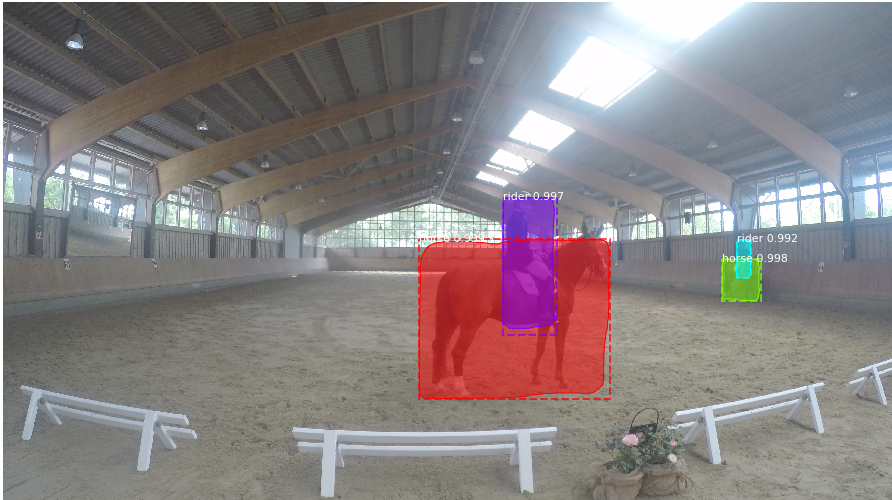
\includegraphics[height=4cm,trim={12cm 0 3cm 0},clip]{./img/IndoorMaske.png}
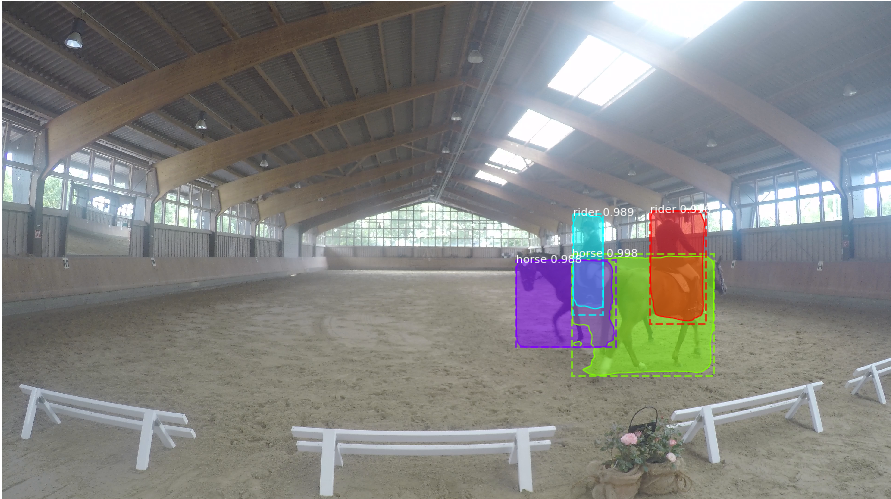
\includegraphics[height=4cm,trim={15cm 0 0 0},clip]{./img/IndoorMaske2.png}
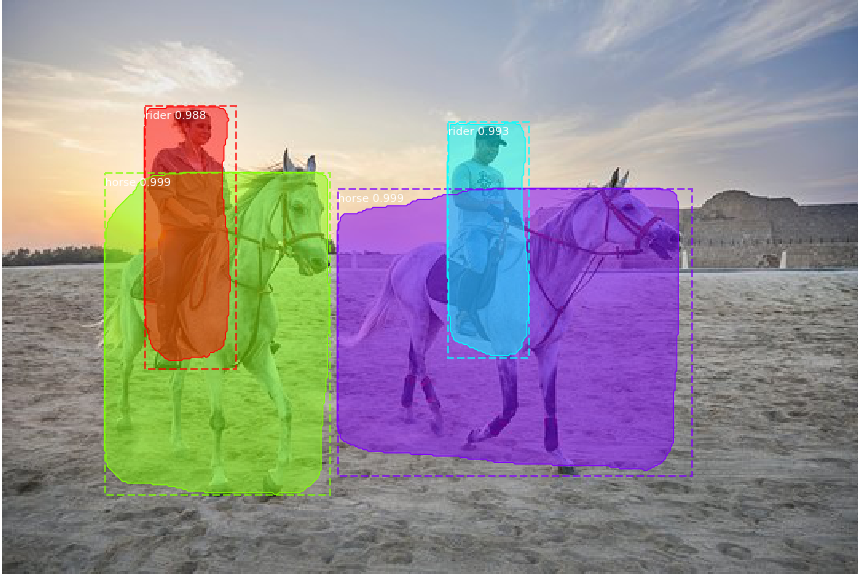
\includegraphics[height=4cm,trim={1cm 0 3cm 0},clip]{./img/OutdoorMaske.png}
\caption{Segmentierung von Reiter und Pferd nach dem Training der zweiten Phase}
\label{fig:SegmentierungPhase2}
\end{figure}

Zur vielfältigen Nutzung des erstellten Detektors, haben wir das Training mit weiteren gelabelten Bilddaten ermöglicht, um den Detektor auch in anderen Hallen zuverlässiger verwenden zu können. Dazu werden die Bilder eines Ordners nacheinander angezeigt, wobei die detektierten Pferde und Reiter mit farbigen Bounding Boxen eingezeichnet werden. Anhand dieser Boxen kann der Nutzer entscheiden, ob die Daten geeignet sind, sodass die akzeptierten Bilder und deren Boxen wie in der Ordnerstruktur von \ref{fig:folderstructure} wiederum abgespeichert werden, um den Detektor damit weiter zu trainieren.

\subsection*{Extraktion der Rois}

Mithilfe von OpenCV werden alle Frames des Eingabevideos einzeln durchlaufen und der zuvor trainierte Detektor auf jedes einzeln angewandt. Dadurch haben wir pro Frame alle erkannten Reiter und Pferde mittels Bounding Boxen abgespeichert und anhand dieser weiter die Rois berechnet, da unser Fokus aus Zeitgründen noch nicht auf Erkennung von Reiterpaaren lag. Wir verfolgten hier den Ansatz zunächst alle Reiter und Pferde in den Rois abzubilden und erst in der dritten Phase zu selektieren um auf ein einzelnes Paar zu fokussieren. Dieser Modus kann weiterhin gut für Aufwärmphasen der Reitturniere genutzt werden, bei denen mehrere Reiterpaare auf dem Turnierplatz sind. Die Umsetzung ist als austauschbarer Filter konzipiert, der eine Gesamt-Bounding-Box anhand der maximalen und minimalen Eckpunkte aller detektierten Bounding-Boxen bestimmt.
Ausgehend von der Gesamt-Bounding-Box müssen für die Erstellung erster Videos noch nötige Sonderfälle beachtet werden. So wird der Zoom unter 480 Pixel verhindert, um eine gute Bildqualität zu ermöglichen. Die längere Seite der Bounding-Box ist ausschlaggebend für die Berechnung der passenden Ratio des Bildausschnittes, sodass dann die optimalen  Eckpunkte berechnet werden können. Wichtig ist es noch die Ränder eines Frames zu berücksichtigen und die Ratio entsprechend zu korrigieren.
Im letzten Schritt werden die Rois mithilfe der kalkulierten Gesamtbox aus jedem Frame ausgeschnitten  . Nachdem alle Frames auf die gleiche Größe gebracht werden, was durch die gleiche Ratio aller Frames keine Verzerrung zur Folge hat, werden die Frames mit OpenCV in ein Ausgabevideo geschrieben.

\todo{Reiterpaare}




\section{Phase 3}
\subsection*{Weiterentwicklung des Detektors}

\begin{figure}[b]
\centering
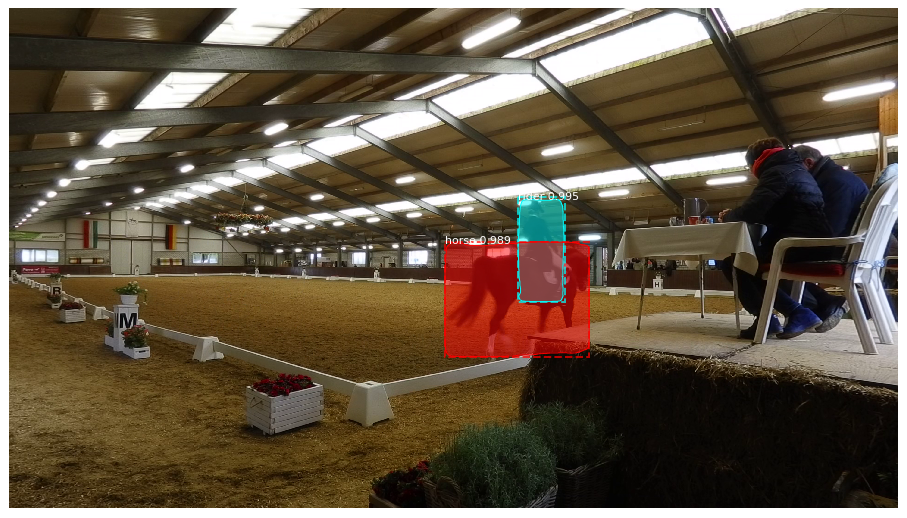
\includegraphics[height=4cm,trim={6cm 0 6cm 0},clip]{./img/IndoorMask6.png}
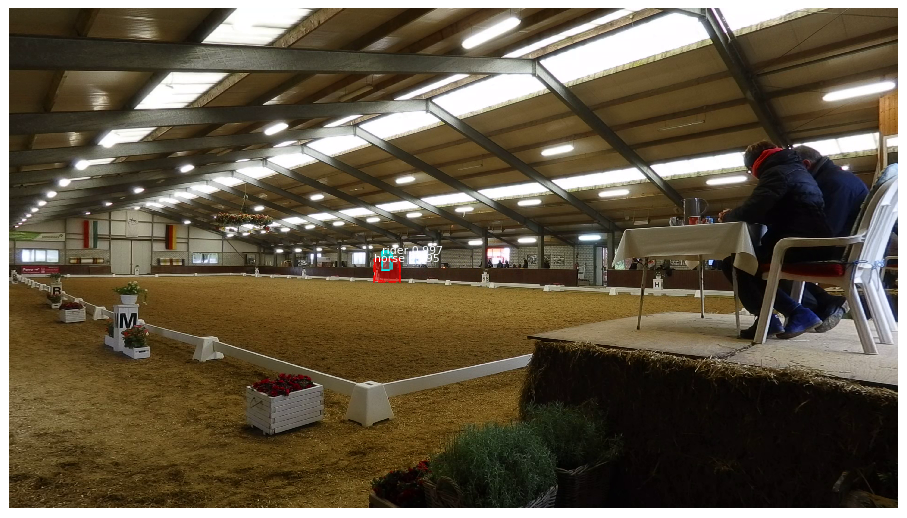
\includegraphics[height=4cm,trim={6cm 0 6cm 0},clip]{./img/IndoorMask3.png}
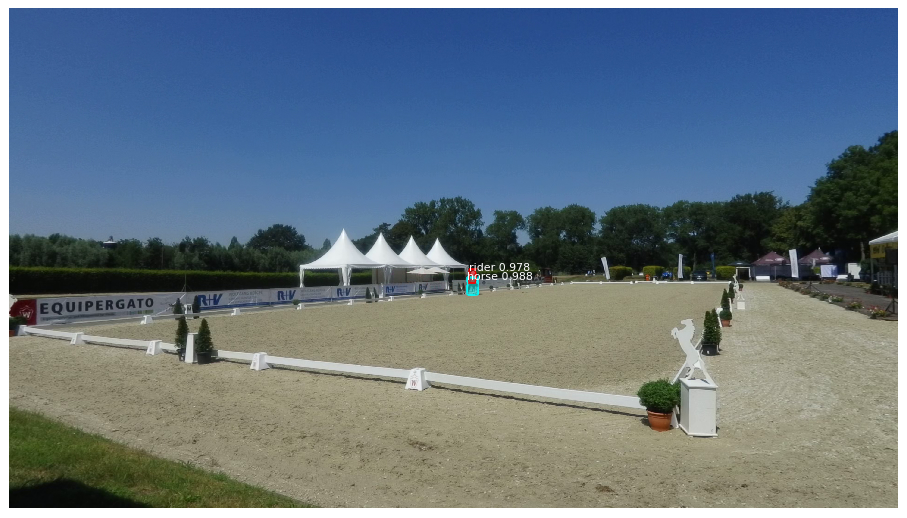
\includegraphics[height=4cm,trim={6cm 0 6cm 0},clip]{./img/OutdoorMask2.png}
\caption{Segmentierung von Reiter und Pferd nach dem Training der zweiten Phase}
\label{fig:SegmentierungPhase3}
\end{figure}

Mit Beginn der dritten Phase wurden weitere Reitvideos zur Verfügung gestellt, welche in verschiedenen Hallen sowie im Außenbereich gefilmt wurden. Der erste Test mit dem Detektor der zweiten Phase verlief nicht sonderlich zufriedenstellend, wodurch wir mehrere Probleme identifizieren konnten. Zum einen wurden nicht alle Reiter und Pferde, die weit entfernt von der Kamera waren, korrekt detektiert. Dieses Ergebnis war aufgrund des zuvor recht einseitigen Trainings nicht verwunderlich, da sich die Hintergründe, Reiter und Pferde unterschieden. Zum anderen wurden auch viele sitzende Personen als Reiter identifiziert und einige Gegenstände wie beispielsweise Pflanzen als fehlerhaft erkannt. Nachdem wir jedoch ungefähr 100 weitere Frames pro neuer Umgebung ausgewählt und damit den Detektor weiter trainiert hatten, wurden ein Großteil der Fehler beseitigt (siehe \ref{fig:SegmentierungPhase3}).


\subsection*{Benutzeroberfläche}

Im Hinblick auf die Kundengruppe haben wir das Kennzeichnung weiterer Bilddaten und die Konvertierung eines Videos für autonome Kameraführung in eine GUI eingebunden. Die GUI wurde mit PyQt5 erstellt und das Standardaussehen durch Einbinden eines Stylesheets modifiziert. Mit dieser minimalen Benutzeroberfläche kann der Nutzer nun zunächst auswählen ob weitere Daten gelabelt werden sollen oder ein Video umgewandelt werden soll. Bei der Auswahl weiter Bilddaten können sowohl Ordner mit Bildern als auch Videos mithilfe extrahierter Frames verwendet werden. Dazu kann der Nutzer pro Bild entscheiden ob die eingezeichnete Detektion gut genug ist diese akzeptieren oder ablehnen und im Anschluss den Detektor damit weiter trainieren. Für die Umwandlung eines Videos wird nach Auswahl der Datei und der Auflösung des Ausgabeformates ein Video unseres Smart Camera Operators erstellt.
\todo{Screenshots Gui Start, Gui Labelling, Gui Convert}

\subsection*{Reiterpaar}
\subsection*{Sprünge/Verschwinden}
\subsection*{Verdecken}
